\subsection{Architecture de l'application}
Notre application web est construite en deux parties distinctes pour séparer la logique de présentation de la logique métier.\\

La partie Front-End utilise Vue.js, un framework JavaScript progressif, pour créer une interface utilisateur intuitive et réactive. Le code est organisé en composants avec des fonctions spécifiques pour améliorer la lisibilité et la maintenance du code.\\

La partie Back-End utilise Flask, un framework Web minimaliste pour Python. Cette partie gère la logique métier et interagit avec la base de données SQLite. Le code, ici encore, est organisé en modules spécifiques pour faciliter la maintenance, en utilisant les blueprints de Flask. Cette approche modulaire permet également d'améliorer la lisibilité et la maintenance du code.\\

La communication entre les deux parties se fait via des appels HTTP pour récupérer, créer, modifier et supprimer des données. Nous avons également utilisé les sockets de Socket.io pour permettre une communication en temps réel entre les deux parties, notamment pour les diffusions des séquences.

\vspace{5mm}
\begin{figure}[H]
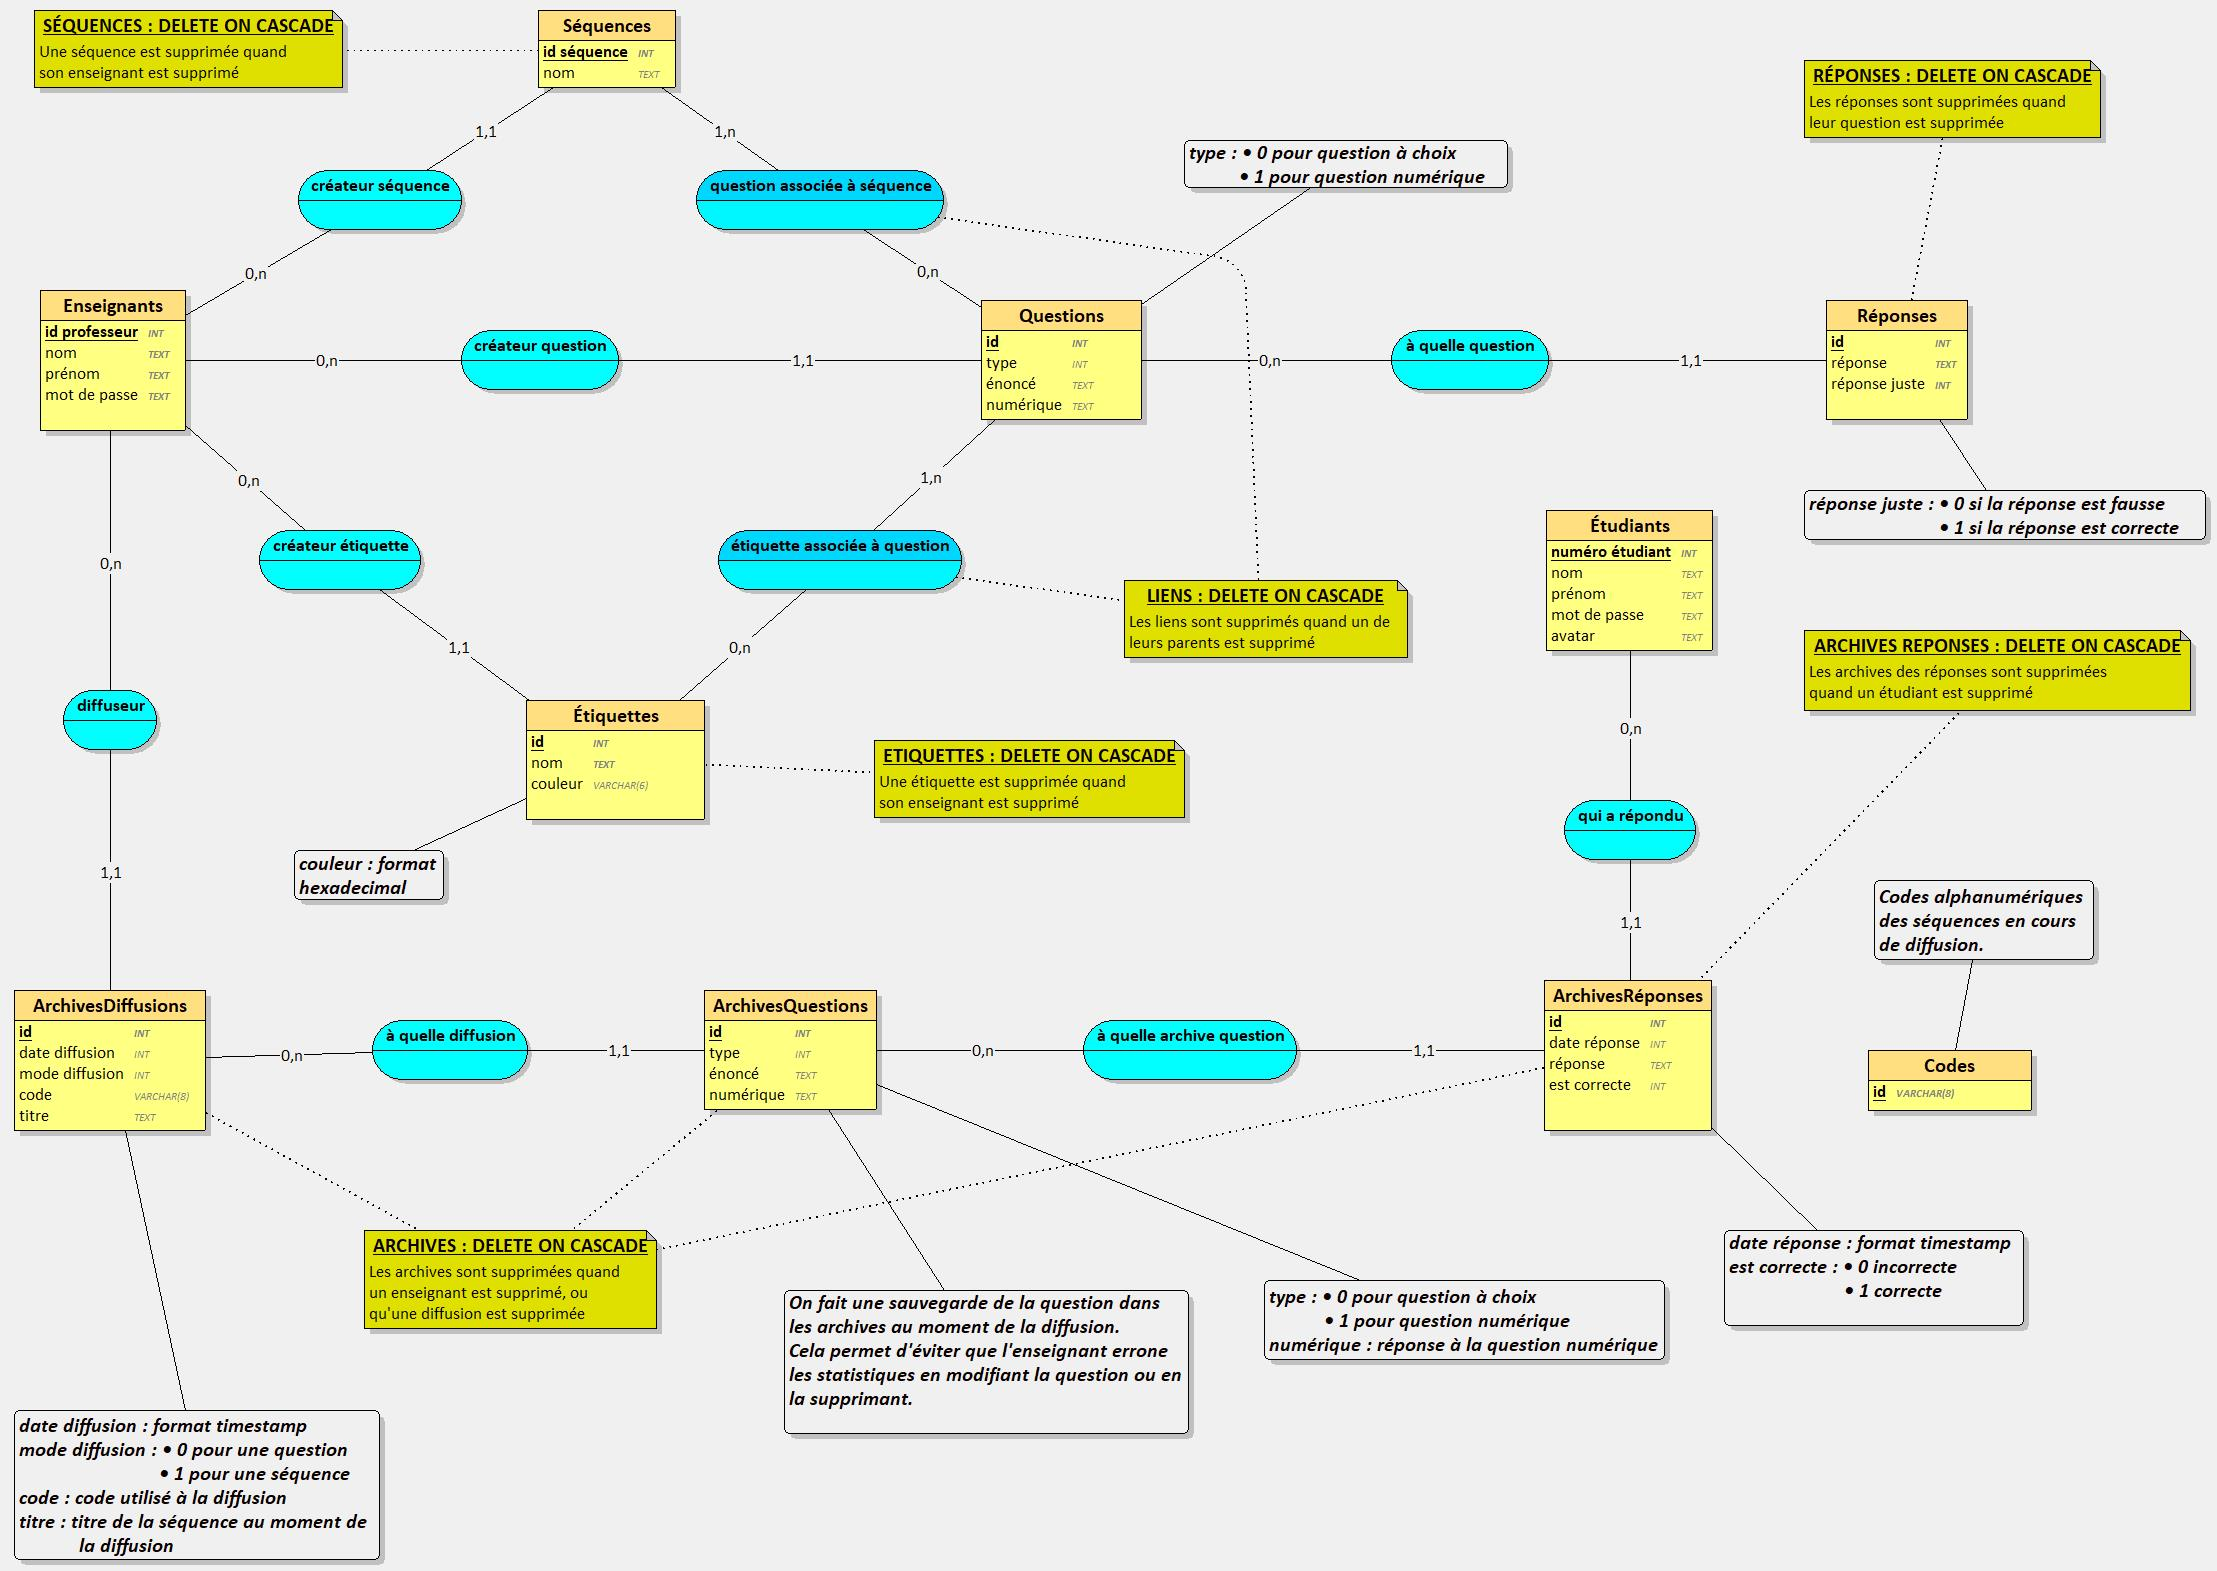
\includegraphics[width=\textwidth]{SchemaBDD.jpg}
\caption{Schéma de la base de données SQLite}
\end{figure}
\vspace{2mm}

\subsection{Choix techniques}
Le choix des technologies pour le développement d'un projet est crucial pour sa réussite. Dans cette partie, nous expliquerons les choix que nous avons faits pour notre application web.

\vspace{2mm}
\subsubsection{Flask : une architecture à base d'API}
Le choix d'utiliser Flask en tant que framework pour notre projet a été imposé par les contraintes du projet. Cependant, nous avons décidé de limiter son utilisation au strict minimum en ne l'utilisant que comme une API. Cette architecture présente de nombreux avantages, tels que la clarté de la séparation entre la logique métier et la présentation, comme mentionné précédemment. Cette séparation facilite grandement le développement en équipe et la maintenance des deux parties de manière indépendante, ce qui rend également l'application plus évolutive. Dans notre cas, où les différentes parties du projet sont découvertes au fur et à mesure, cette évolutivité est essentielle. 

\vspace{2mm}
\subsubsection{Base de données SQLite : avantages par rapport aux fichiers textes}
Nous avons soigneusement étudié plusieurs options de stockage de données, en évaluant leurs avantages et inconvénients respectifs. Après une analyse approfondie, nous avons décidé d'adopter une base de données SQLite.\\

L'utilisation d'une base de données présente de nombreux avantages, notamment une gestion efficace des données et une manipulation aisée. De plus, elle permet une structuration logique et cohérente des données, garantissant ainsi leur intégrité et évitant les erreurs de manipulation.\\

Outre les avantages précités, ce choix nous a permis de mettre en pratique les connaissances acquises lors du troisième semestre.

\vspace{2mm}
\subsubsection{Vue.js : un framework rapide et réactif}
Pour le développement de la partie Front-End de notre application, nous avons opté pour Vue.js. Et ce pour plusieurs raisons;
Nous avons tout d'abord été séduits par la rapidité du framework ainsi que sa réactivité. Ces deux avantages nous ont permis de créer rapidement une interface utilisateur intuitive et réactive.\\

Un autre avantage de Vue.js est sa facilité d'utilisation, en particulier pour les membres de l'équipe qui n'avaient pas d'expérience préalable avec des frameworks JavaScript. C'est Donovann qui a proposé Vue.js en raison de ses connaissances solides en React et de son désir de découvrir un nouveau framework.\\

Enfin, l'utilisation de Vue.js avec Flask nous a permis d'optimiser la vitesse de l'application, ce qui est un avantage considérable pour une application Web.